\documentclass[tikz,border=10pt]{standalone}
\usepackage{tikz}
\usetikzlibrary{arrows.meta,positioning}
\definecolor{bg}{HTML}{171D2B}
\definecolor{accent}{HTML}{F7B538}
\definecolor{tealsoft}{HTML}{2DD4BF}
\definecolor{salmon}{HTML}{F97066}
\pagecolor{bg}
\color{white}

\begin{document}
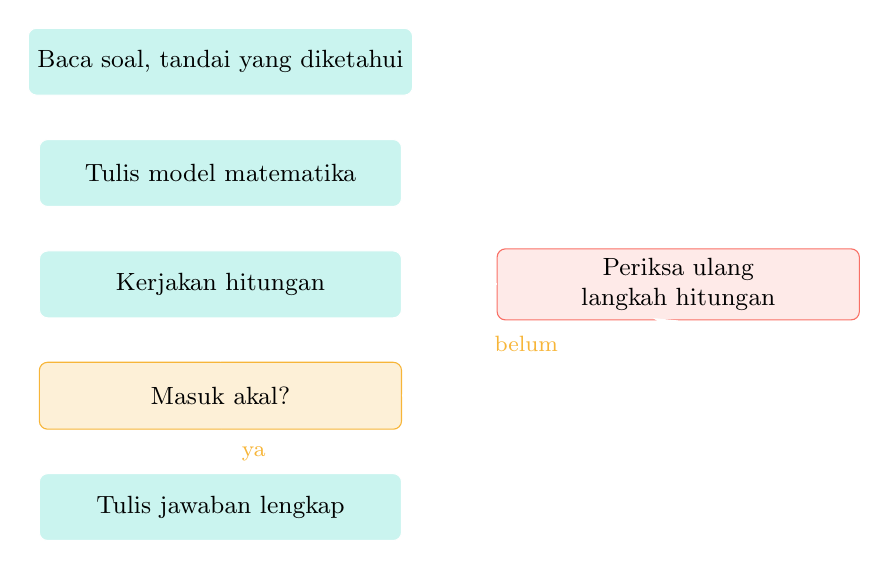
\begin{tikzpicture}[
  node distance=0.55cm and 0.5cm,
  kotak/.style={rectangle, rounded corners=3pt, draw=white, fill=tealsoft!25,
    minimum width=4.6cm, minimum height=0.85cm, align=center, font=\small},
  keputusan/.style={rectangle, rounded corners=3pt, draw=accent, fill=accent!20,
    minimum width=4.6cm, minimum height=0.85cm, align=center, font=\small},
  teks/.style={font=\small\color{white}},
  panah/.style={-{Stealth[length=3mm]}, draw=white, thick},
  cabang/.style={font=\footnotesize\color{accent}}
]

\node[kotak] (baca) {Baca soal, tandai yang diketahui};
\node[kotak, below=of baca] (model) {Tulis model matematika};
\node[kotak, below=of model] (hitung) {Kerjakan hitungan};
\node[keputusan, below=of hitung] (cek) {Masuk akal?};
\node[kotak, below=of cek] (tulis) {Tulis jawaban lengkap};
\node[kotak, right=1.2cm of hitung, draw=salmon, fill=salmon!15] (ulang) {Periksa ulang\\langkah hitungan};

\draw[panah] (baca) -- (model);
\draw[panah] (model) -- (hitung);
\draw[panah] (hitung) -- (cek);
\draw[panah] (cek) -- node[cabang, right=4pt, pos=0.55] {ya} (tulis);
\draw[panah] (cek.east) -- node[cabang, pos=0.45, above] {belum} (ulang.south);
\draw[panah] (ulang.west) -- (hitung.east);

\end{tikzpicture}
\end{document}
